\documentclass[a4paper]{article}

% Set margins
\usepackage[hmargin=2cm, vmargin=2cm]{geometry}

\frenchspacing

% Language packages
\usepackage[utf8]{inputenc}
\usepackage[T1]{fontenc}
\usepackage[magyar]{babel}

% AMS
\usepackage{amssymb,amsmath}

% Graphic packages
\usepackage{graphicx}

% Colors
\usepackage{color}
\usepackage[usenames,dvipsnames]{xcolor}

% Enumeration
\usepackage{enumitem}

\usepackage{listings}
\usepackage{python}
\usepackage{hyperref}

\begin{document}

\noindent \textbf{Szakdolgozat II. -- A folyamatmodellező gráf leírása}

\vskip 8mm

Az alkalmazás részeinek megtervezéséhez különböző üzleti folyamatoknak jártam utána, hogy lássam, milyen elemekből épül fel egy ilyen gráfszerkesztő. Elsőként egy egyszerűbb ábrát találtam, ami azt modellezi, hogy hogyan készül el egy megrendelt pizza az étteremben.

\begin{figure}[h]
\centering
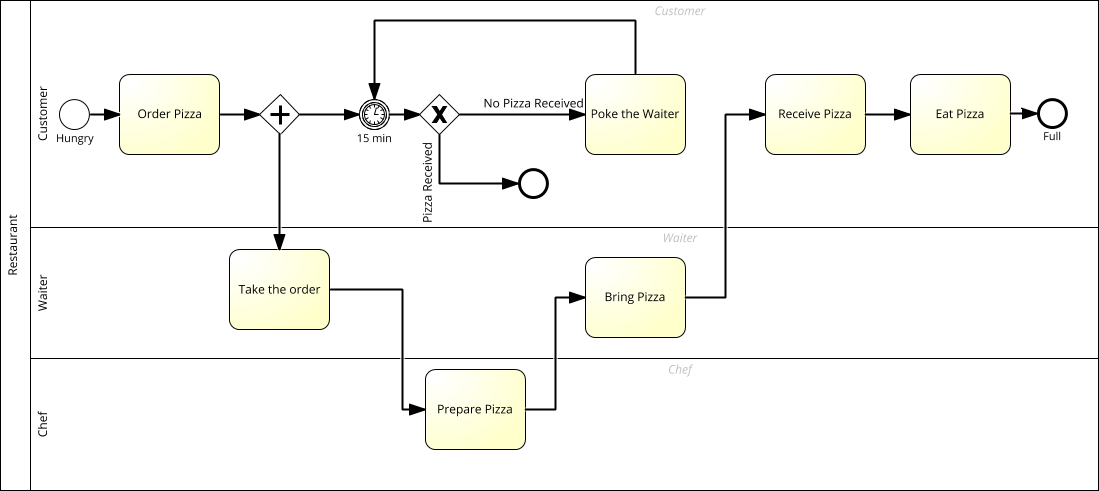
\includegraphics[width=16truecm]{pizzarest.png}
\caption{Készül a pizza}
\end{figure}

Látható, hogy a már meglévő gráfszerkesztőmet további elemekkel kell kiegészíteni. Ezen elemek pontos neveinek utánajárva az alábbi adatfolyam elemekkel egészítem ki a gráfszerkesztőt:
\begin{itemize}
\item Kezdő- és végesemény definiálására kör alakú elemek (különböző vastagsággal aszerint, hogy az start vagy stop esemény)
\item Tevékenységek definiálása (lekerekített téglalap). Ebből van a legtöbb a gráfban, hiszen ezek szemléltetik magát a folyamatot, az események egymás utáni történését. Ezek jelenleg csomópont (\textit{node}) néven vannak definiálva.
\item Átjárók bevezetése (rombusz alak). Ezek gyakorlatilag logikai kapukként (\textit{OR, AND, XOR...}) funkcionálnak, vagyis akkor használatosak, amikor egy elágazás következik a folyamatábrán.
\end{itemize}

Ezeken kívül látható, hogy a nyilakon, illetve a tevékenységekben szövegek is előfordulnak. Ezek fontos szerepet töltenek be a gráfszerkesztőnél, hiszen információkat hordoznak az adott állapotról. Természetesen ezeket tudnia kell a felhasználónak tetszés szerint megadnia illetve módosítania.

Látható még egy óra szimbólum is a folyamatábrán. Ez akkor használatos, amikor ki akarjuk emelni két esemény között az eltelt időt. Itt szintén a felhasználó adhatja meg percben, hogy mennyi legyen az a bizonyos idő.

A tagolás kétféleképpen történik. Kívül jelöljük a résztvevőt (ún. \textit{pool}ban - itt az étterem), azon belül pedig sávok (ún. \textit{lane}) szerint csoportosítjuk a tevékenységeket. így elkülönül a vevő, aki megrendeli, szükség esetén megsürgeti, megkapja, majd elfogyasztja a pizzát. Továbbá a pincér, aki felveszi a megrendelést, és teljesíti azt. Valamint a szakács, aki elkészíti a pizzát.

A nyilak, amik az összeköttetést valósítják meg az adatfolyam elemei között, nem csak egyenesen rámutatnak az egyik tevékenységről a másikra, hanem meg is törnek. Ezt többféleképpen is lehet kivitelezni:

\begin{itemize}
\item Az ábrán látható módon 90 fokos szögben elhajlanak, ahol szükséges.
\item A nyíl útvonala egy görbét ír le.
\end{itemize}

Alapvetően ilyen elemtípusokból épül fel egy egyszerűbb modellező folyamatábra (angol megfelelője a \textit{BPMN - Business Process Model and Notation}).

Mielőtt konkrét, üzleti folyamatok modellezését vizsgáljuk, nézzünk egy másik példát, ahol a fogyasztó egy pizzafutártól rendel pizzát.

\newpage

\begin{figure}[h]
\centering
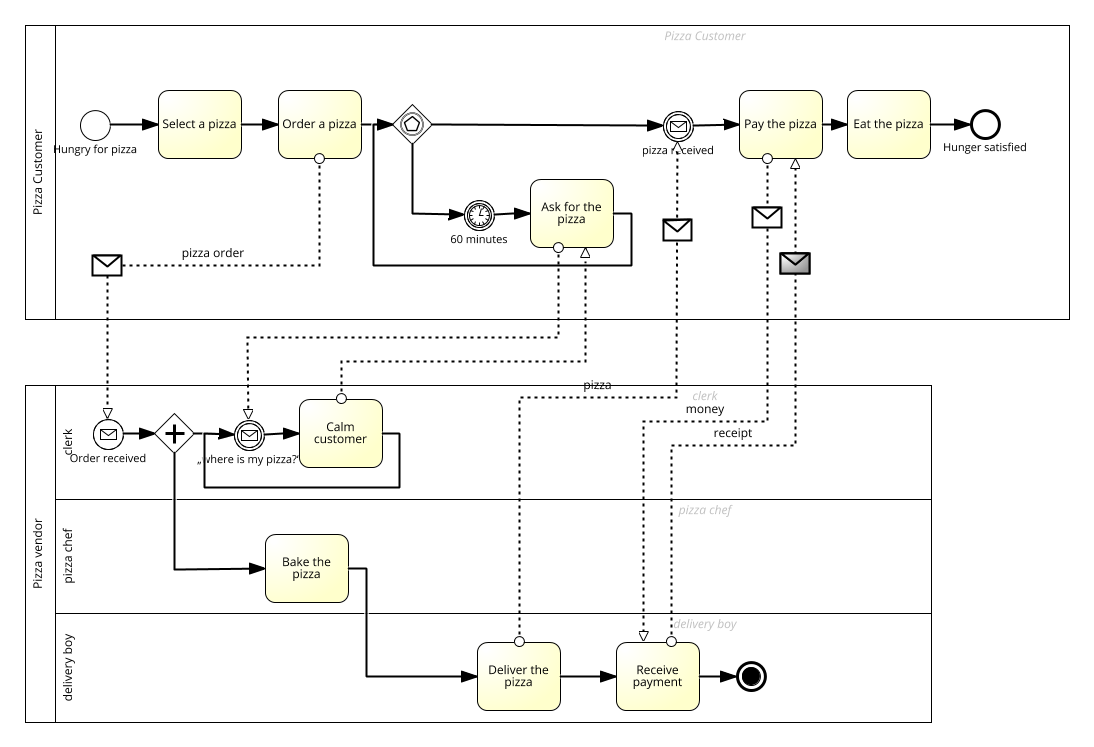
\includegraphics[width=16truecm]{pizzadeliv.png}
\caption{Futár hozza a pizzát}
\end{figure}

Látható, hogy itt már összetettebb folyamatról van szó (például két résztvevő van), azonban nem sokkal több az új elem az előzőhöz képest.

\begin{itemize}
\item Megjelenik a szaggatott vonalas nyíl (az \textit{üzenet}). Ez egy információcsere két független folyamat résztvevő között, tehát két különálló \textit{pool} elemeit köti össze.
\item Az üzenet szintén egy új elembe kapcsolódik be, az üzenet csomópontba.
\item Itt már nem a klasszikus egy bemenet - egy kimenet figyelhető meg, hiszen a folyamatot a vevő megrendelése indítja el, és a vevő, valamint a pizza eladó külön-külön zárja le. Pontosabban a vevő befejezi a folyamatot (\textit{befejező esemény jel}) azzal, hogy elfogyasztja a rendelt terméket, a pizza szolgálat pedig \textit{terminálja} az egész folyamatot. A terminálásnak külön jelölése van.
\end{itemize}

Források:
\begin{itemize}
\item 1, 2. ábra: \url{https://training-course-material.com/training/BPMN_2.0_Example_-_Pizza}
\item 3. ábra: Nincs még
\end{itemize}

\begin{python}
<canvas id="my-canvas" width="800" height="600">
\end{python}

\end{document}